% --------------------------------------------------------------
% This is all preamble stuff that you don't have to worry about.
% Head down to where it says "Start here"
% --------------------------------------------------------------
 
\documentclass[12pt]{article}
 
\usepackage[margin=1in]{geometry} 
\usepackage{mathtools}
\usepackage{bm}
\usepackage{subfig}
\usepackage{amssymb}

\setlength{\parskip}{1em}

% \newenvironment{theorem}[2][Theorem]{\begin{trivlist}
% \item[\hskip \labelsep {\bfseries #1}\hskip \labelsep {\bfseries #2.}]}{\end{trivlist}}
% \newenvironment{lemma}[2][Lemma]{\begin{trivlist}
% \item[\hskip \labelsep {\bfseries #1}\hskip \labelsep {\bfseries #2.}]}{\end{trivlist}}
% \newenvironment{exercise}[2][Exercise]{\begin{trivlist}
% \item[\hskip \labelsep {\bfseries #1}\hskip \labelsep {\bfseries #2.}]}{\end{trivlist}}
% \newenvironment{reflection}[2][Reflection]{\begin{trivlist}
% \item[\hskip \labelsep {\bfseries #1}\hskip \labelsep {\bfseries #2.}]}{\end{trivlist}}
% \newenvironment{proposition}[2][Proposition]{\begin{trivlist}
% \item[\hskip \labelsep {\bfseries #1}\hskip \labelsep {\bfseries #2.}]}{\end{trivlist}}
% \newenvironment{corollary}[2][Corollary]{\begin{trivlist}
% \item[\hskip \labelsep {\bfseries #1}\hskip \labelsep {\bfseries #2.}]}{\end{trivlist}}
\newenvironment{question}[2][Question]{\begin{trivlist}
\kern10pt
\item[\hskip \labelsep {\bfseries #1}\hskip \labelsep {\bfseries #2.}]}{\end{trivlist}}


\newcommand\TODO[1]{\textcolor{red}{#1}}

\begin{document}
 
% --------------------------------------------------------------
%                         Start here
% --------------------------------------------------------------
 
%\renewcommand{\qedsymbol}{\filledbox}
 
\title{DD2434 Machine Learning, Advanced Course Assignment 1}
\author{Lin Chun Hung, chlin3@kth.se} 
 
\maketitle


% Question 1
\begin{question}{1}
% TODO: Fix the arguments
Consider input output pairs are linked by the mapping to have the following
 relation:
$$ 
    \bf{t}_i = f(\bf{x}_i) + \bm{\epsilon}
$$
where the $\bm{\epsilon}$ is the unbiased random noise. Since we have no piror knowledge
on the random noise term, the random noise is then assumed as following the normal
distribution. TODO: More on this \par

With the assumption that features are uncorrelated, we choose the spherical
covariance matrix for the likelihood.
\end{question}
% End question 2



% Question 2
\begin{question}{2}
Consider the general product rule of probability:
$$\mathrm {P} \left(\bigcap _{k=1}^{n}A_{k}\right)=
  \prod _{k=1}^{n}\mathrm {P} \left(A_{k}\,{\Bigg |}\,\bigcap _{j=1}^{k-1}A_{j}\right)$$

Therefore the likelihood would be:
$$ 
  p(\bf{T}\mid f,\bf{X}) =
  \prod _{i=1}^{N}p(\bf{t}_i \mid \bf{t}_{i-1},...,\bf{t}_{1},
  f,\bf{X})
$$

\end{question} 
% End question 2


% Question 3 
\begin{question}{3}

$$ 
  p(\bf{T}\mid \bf{X},\bf{W}) =
  \prod _{i=1}^{N}N(\bf{W}\bf{x}_i, \sigma^2\bf{I})
$$

\end{question}
% End question 3

% Question 4
\begin{question}{4}
The choice of piror distribution reflects the choice of regularizer. Chossing L1 
norm as regularizer is known as the lasso (least absolute shrinkage and selection operator).
The regularizer will force some weighting coefficients $w_j$ to be zero, given 
a proper choice of model parameter $\tau$. It plays the role of feature selection
since those zero weighting coefficients indicate that the corresponding features
are irrelvant to the output. \par

The penalization term or the negative log-prior:
$$  \frac{\lambda}{2} \left \|\textbf{vec}(\bf{W} - \bf{W}_0)\right \|_{q}  $$

\begin{figure}[h!]
  \centering
  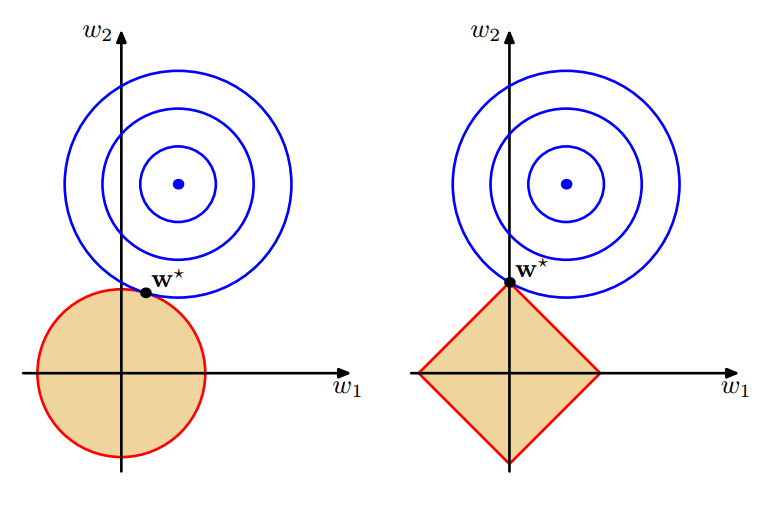
\includegraphics[width=0.5\linewidth]{q4_regular.png}
  \caption{A boat.}
  \label{fig:boat1}
\end{figure}

TODO: Discussion
\end{question}
% End question 4



% Question 5
\begin{question}{5}
TODO: Add dimension\\
Consider the regression equation in general:
$$\textbf{T} = \textbf{WX} + \textbf{ErrorMatrix} $$
Therefore, the likelihood in terms of matrix normal distribution is:
\begin{align*}
p(\bf{T}\mid \bf{X}, \bf{W}) &= 
  \mathcal{MN}_{D \times N}(\bf{WX}, \bf{I}, \sigma^2 \bf{I}) \\ 
  &= \mathcal{N}_{DN}(\bf{vec}(\bf{WX}), \sigma^2 \bf{I})
\end{align*}
The prior is:
\begin{align*}
p(\bf{W}) &= 
  \mathcal{MN}_{D \times q}(\textbf{W}_0, \bf{I}, \tau^2 \bf{I}) \\
  &= \mathcal{N}_{Dq}(\textbf{vec}(\textbf{W}_0), \tau^2 \bf{I})
\end{align*}

Due to the choice of a conjugate Gaussian prior distribution, the posterior will 
also be Gaussian:
$$
p(\textbf{W}\mid \textbf{X}, \textbf{T}) =
  \mathcal{N}_{Dq}(\textbf{vec}(\textbf{W}_{p0}), \bm{\Sigma}_{p0} )
$$

To calculate the mean and covariance of the posterior over the parameters,
Consider the equation 7 in the question with respect to the parameters $\textbf{W}$
 and compare the quadratic and linear terms of the exponents in both sides:
\begin{align*}
  p(\textbf{W}\mid \textbf{X}, \textbf{T}) =&
  \frac{1}{Z}p(\textbf{T}\mid \textbf{X}, \textbf{W})p(\textbf{W})  \\
  \ln p(\textbf{W}\mid \textbf{X}, \textbf{T}) =&
  \ln p(\textbf{T}\mid \textbf{X}, \textbf{W}) + \ln p(\textbf{W}) + \text{Const.} \\
\end{align*}
\begin{align*}
  LHS =& -\frac12[\textbf{vec}(\textbf{W}) - \textbf{vec}(\textbf{W}_{p0)}]^T
          \bm{\Sigma}_{p0}^{-1}[\textbf{vec}(\textbf{W})-\textbf{vec}(\textbf{W}_{p0})] \\
  RHS =& -\frac{1}{2\sigma^2}[\textbf{vec}(\textbf{T}) - \textbf{vec}(\textbf{WX})]^T
                             [\textbf{vec}(\textbf{T}) - \textbf{vec}(\textbf{WX})] \\
       &-\frac{1}{2\tau^2}[\textbf{vec}(\textbf{W}) - \textbf{vec}(\textbf{W}_0)]^T
                          [\textbf{vec}(\textbf{W}) - \textbf{vec}(\textbf{W}_0)]
\end{align*}

Consider the quadratic terms on both sides:
\begin{equation} \label{eq:q5-covar}
  \begin{aligned}[b]
    -\frac12\textbf{vec}(\textbf{W})^T\bm{\Sigma}_{p0}^{-1}\textbf{vec}(\textbf{W})
    =& -\frac{1}{2\sigma^2}\textbf{vec}(\textbf{WX})^T\textbf{vec}(\textbf{WX})
    -\frac{1}{2\tau^2}\textbf{vec}(\textbf{W})^T\textbf{vec}(\textbf{W}) \\
    -\frac12\textbf{vec}(\textbf{W})^T\bm{\Sigma}_{p0}^{-1}\textbf{vec}(\textbf{W})
    =& -\frac{1}{2\sigma^2}\textbf{vec}(\textbf{W})^T(\mathbf{X}^T \otimes \mathbf{I}_D)^T
    (\mathbf{X}^T \otimes \mathbf{I}_D)\textbf{vec}(\textbf{W}) \\
    & -\frac{1}{2\tau^2}\textbf{vec}(\textbf{W})^T\textbf{vec}(\textbf{W}) \\
    -\frac12\bm{\Sigma}_{p0}^{-1} =&
    -\frac{1}{2\sigma^2}(\mathbf{X} \otimes \mathbf{I}_D)(\mathbf{X}^T \otimes \mathbf{I}_D) 
    -\frac{1}{2\tau^2} \mathbf{I}_{Dq}\\
    \bm{\Sigma}_{p0}^{-1} =& \hspace{5mm} 
    \frac{1}{\sigma^2}(\mathbf{X}\mathbf{X}^T)\otimes \mathbf{I}_D +\frac{1}{\tau^2}\mathbf{I}_{Dq}
  \end{aligned}
\end{equation}

Consider the linear terms on both sides:  
\begin{align*}
    \textbf{vec}(\textbf{W})^T\bm{\Sigma}_{p0}^{-1}\textbf{vec}(\textbf{W}_{p0})
    =& \hspace{1mm} 
       \frac{1}{\sigma^2}\textbf{vec}(\textbf{WX})^T\textbf{vec}(\textbf{T}) 
     + \frac{1}{\tau^2}\textbf{vec}(\textbf{W})^T\textbf{vec}(\textbf{W}_0)\\
    \textbf{vec}(\textbf{W})^T\bm{\Sigma}_{p0}^{-1}\textbf{vec}(\textbf{W}_{p0})
    =& \hspace{1mm} 
       \frac{1}{\sigma^2}\textbf{vec}(\textbf{W})^T(\mathbf{X}\otimes\mathbf{I}_D)
       \textbf{vec}(\textbf{T}) 
     + \frac{1}{\tau^2}\textbf{vec}(\textbf{W})^T\textbf{vec}(\textbf{W}_0)\\
    \textbf{vec}(\textbf{W}_{p0}) =& \hspace{1mm} 
       \bm{\Sigma}_{p0}[\frac{1}{\sigma^2}(\mathbf{X}\otimes\mathbf{I}_D)
       \textbf{vec}(\textbf{T}) + \frac{1}{\tau^2}\textbf{vec}(\textbf{W}_0)] \\
\end{align*}
\begin{equation} \label{eq:q5-mean}
    \textbf{vec}(\textbf{W}_{p0}) =
    [\frac{1}{\sigma^2}(\mathbf{X}\mathbf{X}^T)\otimes \mathbf{I}_D +\frac{1}{\tau^2}\mathbf{I}_{Dq}]^{-1}
       [\frac{1}{\sigma^2}(\mathbf{X}\otimes\mathbf{I}_D)
       \textbf{vec}(\textbf{T}) + \frac{1}{\tau^2}\textbf{vec}(\textbf{W}_0)]
\end{equation}

Consider an infinitely broad prior, which means $\tau \to \infty$, reduces the 
mean and covariance of the posterior to the mean and covariance of the likelihood
estimated under maximum likelihood approach. \par

The constant $Z$ plays no role in the calculation since only the quadratic and linear
 terms are considered.
% Subsitute back \eqref{eq:q5-covar} and \eqref{eq:q5-mean} into the posterior

\end{question}
% End question 5

% Question 6
\begin{question}{6}
\begin{align*}
  p(f\mid X,\theta) = N(0, k(X, X))  % TODO: fix this equation
\end{align*}
  The prior distribution over functions expresses our beliefs and knowledge about
how the function looks like before we consider the data.

We choose the mean function as zero or the instaniation of function to be zero
 since we have forced the data to have zero-mean. We can choose a non-zero mean
 function of the Gaussian process. Indeed, we can use a fixed mean function, but
 the result is trivial that we can obtain the predictive mean function by adding 
 the mean-removal result to the fixed mean function.
 (Rasmussen, C. E., 2004, page 27)

The covariance of the marginal distribution, which is the prior, is the covariance
function controlled by the hyperparameter $\bm{\theta}$. The covariance function
tells that if two input points are similar, then the output should be similar as
well. The specification of the covariance function indicates a distribution over 
functions. To visualize it, we can draw some smaples from the distribution of 
function evaluated at some input points.

%TODO: Fix this figure, use python to replot it
\begin{figure}[h!]
  \centering
  \includegraphics[width=0.5\linewidth]{q6_output_prior.png}
  \caption{fix me!}
  \label{fig:fix me!}
\end{figure}
\end{question}

% Question 7
\begin{question}{7}
  \begin{align*}
    p(\mathbf{T}, \mathbf{X}, f, \bm{\theta}) 
      = p(\mathbf{T}\mid f)p(f \mid \mathbf{X},\bm{\theta})
      p(\mathbf{X})p(\bm{\theta}) 
  \end{align*}
  TODO: Add graph model
\end{question}

\begin{question}{8}
\begin{align*}
  p(\mathbf{T} \mid \mathbf{X}, \bm{\theta}) = \int p(\mathbf{T}\mid f)p(f) df
\end{align*}

The marginalisation connects the prior and the likelihood of the data. The
 integral is an weighted average which averages the likelihood of the data.
 The weighting is given by the prior which is the probability distribution of
 the function.

The uncertainties of the data and the prior are combined or added up into the 
 uncertainty of the marginalisation. Equation 6.62 of Bishop book (2006 Ed.) shows
 how two uncertainties (covariances) are simplily added up.

The hyperparameters $\bm{\theta}$ still condition on the part of covariance of the 
 marginalisation from the prior. That part of covariance is the kernel function.
\end{question}

\begin{question}{9}
  Practical TODO:
\end{question}

\begin{question}{10}
  Practical TODO:
\end{question}

\begin{question}{11}
  Practical TODO:
\end{question}

\begin{question}{12}
This prior encodes that we have no perference on the latent variable. It just 
 shows that we have no information about the latent variable $X$. Therefore, 
 we assume that it is a zero-mean Gaussian and each compoent are indepenent.
\end{question}

\begin{question}{13}
Consider the linear equation of $\mathbf{Y}(\mathbf{X})$:
  \begin{align*}
    \mathbf{Y}(\mathbf{X}) = \mathbf{W}\mathbf{X} + \bm{ErrorMatrix}
  \end{align*}
And each column of $\mathbf{Y}$ can be written as:
\begin{align*}
  \mathbf{y}_i = \mathbf{W}\mathbf{x}_i + \bm{\epsilon}
\end{align*}
Because $p(\mathbf{X})$ and $p(\mathbf{Y}\mid\mathbf{X}, \mathbf{W})$ are Gaussian, 
 the marginal distribution is also Gaussian.
 Furthermore, we can consider each $\mathbf{y}_i$ are indepenent. Therefore, 
 we can write:
\begin{align*}
  p(\mathbf{Y}\mid\mathbf{W}) &= \prod_{i=1}^{N} p(\mathbf{y}_i\mid\mathbf{W}) \\
  p(\mathbf{y}_i\mid\mathbf{W}) &= N(\mathbf{y}_i\mid \mathbb{E}[\mathbf{y}_i], \text{cov}[\mathbf{y}_i])
\end{align*}
Then, our job is to calculate the mean and covariance of the Gaussian.

Notes that $\mathbf{W}$ is given, $\bm{\epsilon} \sim \mathcal{N}(\mathbf{0}, \sigma^2\mathbf{I})$
 and $\mathbf{x}_i \sim \mathcal{N}(\mathbf{0}, \mathbf{I})$ as 
 $p(\mathbf{X}) = \mathcal{N}(\mathbf{0}, \mathbf{I})$
\begin{align*}
  \mathbb{E}[\mathbf{y}_i] &= \mathbb{E}[\mathbf{W}\mathbf{x}_i + \bm{\epsilon}] \\ 
  &= \mathbb{E}[\mathbf{W}\mathbf{x}_i + \bm{\epsilon}] \\
  &= \mathbf{0} + \mathbf{0} 
                      && (\text{by the prior }\mathbb{E}[\mathbf{x}_i] = \mathbf{0})\\
  &= \mathbf{0} \\
  \text{cov}[\mathbf{y}_i] 
  &= \mathbb{E}[(\mathbf{W}\mathbf{x}_i + \bm{\epsilon})
                (\mathbf{W}\mathbf{x}_i + \bm{\epsilon})^{T}] \\
  &= \mathbb{E}[\mathbf{W}\mathbf{x}_i\mathbf{x}_i^T\mathbf{W}^T]
     + \mathbb{E}[\bm{\epsilon}\bm{\epsilon}^{T}]
     && (\text{noise and }\mathbf{W}\mathbf{x}_i\text{ are uncorrelated}) \\
  &= \mathbf{W}\mathbb{E}[\mathbf{x}_i\mathbf{x}_i^T]\mathbf{W}^T + \sigma^2 \mathbf{I}
     && (\bm{\epsilon} \sim N(\mathbf{0}, \sigma^2\mathbf{I})) \\
  &= \mathbf{W}\mathbf{W}^T + \sigma^2\mathbf{I}
     && (\text{cov}[\mathbf{x}_i] = \mathbf{I})
\end{align*}

The marginal distribution is:
\begin{equation}
  p(\mathbf{Y}\mid\mathbf{W}) 
  = \prod_{i=1}^{N} 
    \mathcal{N}(\mathbf{y}_i\mid\mathbf{0}, \mathbf{C})
\end{equation}
where $\mathbf{C}$ is a covariance matrix defined as:
\begin{align*}
  \mathbf{C} = \mathbf{W}\mathbf{W}^T + \sigma^2\mathbf{I}
\end{align*}
\end{question}

\begin{question}{14}
First, let's write down different estimation in log-space.

Consdier we have a linear relation Y(X) mentioned in Q13.
\\ 
Maximum-likelihood estimation:
\begin{align*}
  \hat{\mathbf{W}} 
  &= \operatorname{argmin}_{\mathbf{W}}
    [\sum_{i=1}^{N} \| \mathbf{y}_i - \mathbf{W}\mathbf{x}_i\|^2]
\end{align*}
It is equivalent to find the parameter with least square method. More data makes
the computational time longer.

Maximum-a-posteriori (MAP) estimation:
\begin{align*}
  \hat{\mathbf{W}} 
  &= \operatorname{argmin}_{\mathbf{W}}
    [\sum_{i=1}^{N} \| \mathbf{y}_i - \mathbf{W}\mathbf{x}_i\|^2
      + \lambda \textbf{vec}(\textbf{W})^T\textbf{vec}(\textbf{W})]
\end{align*}
MAP approach has an extra regularization term for preventing from overfitting.
We have a degree of freedom to choose the regularizer coefficient.
If we have more data, then regularization term will be less important compared
with the least square error term.

Type-II Maximum-Likelihood:
\begin{align*}
  \hat{\mathbf{W}} 
  &= \operatorname{argmin}_{\mathbf{W}}
    [\sum_{i=1}^{N} \mathbf{y}_i^T \mathbf{C}^{-1}\mathbf{y}_i
      + N\log{|\mathbf{C}|}]
\end{align*}
Type-II maximum likelihood approach does not depends on $\mathbf{X}$ and it is
very useful in our case. $N\log{|\mathbf{C}|}$ expresses the model complexity
and $\sum_{i=1}^{N} \mathbf{y}_i^T \mathbf{C}^{-1}\mathbf{y}_i$ plays the role of
goodness of fit. When data become more, the plenalty of the model complexity becomes
more important.
  
The last two expression of Eq. 25 are equivalent. It is because the dominator:
  \begin{align*} % TODO: input the last two integral of eq. 25
    \int p(\mathbf{Y}\mid\mathbf{X}, \mathbf{W})p(\mathbf{W})d\mathbf{W}
  \end{align*}
is not a function of $\mathbf{W}$. And we know that that integral gives a possitive
 real number. Therefore, when finding the maximum value of $\mathbf{W}$, the dominator 
 can be ignored.

The Type-II Maximum-likelihood is a sensible approach since it consider how to
 choose a parameter $\mathbf{W}$ which maximizes the model evidence. In other words,
 it is in the sense that we choose a parameter to maximize the probability of 
 getting such a set of observations.
\end{question}
\begin{question}{15}
  TODO
\end{question}  

% --------------------------------------------------------------
%     You don't have to mess with anything below this line.
% --------------------------------------------------------------
\end{document}
